%!TEX root = ../thesis.tex

% \pagebreak[4]
% \hspace*{1cm}
% \pagebreak[4]
% \hspace*{1cm}
% \pagebreak[4]

\chapter{Déformation à base de cage}

\graphicspath{ {Chapter2/Chapter2Figs/PNG/}
  {Chapter2/Chapter2Figs/PDF/} {Chapter2/Chapter2Figs/} }

Notre travail s'est porté particulièrement sur le mélange de différents outils
à base de surfaces. La technique retenue pour cette dimension est celle
des déformations à base de cage. Ce choix a été motivé par l'efficacité de
cette méthode et de son utilisation dans le travail de \cite{GPCP13} (un
travail similaire à celui que nous souhaitions réaliser).

Ces déformations peuvent se faire dans $\mathbb{R}^2$ (l'outil
est un polygone) et dans $\mathbb{R}^3$ (l'outil est une surface). Pour
simplifier la compréhension de la méthode ainsi que les différents schémas,
nous nous limiterons aux déformations dans $\mathbb{R}^2$.

\section{Introduction} 

L'outil permettant de réaliser les déformations est un polygone. Ce polygone
peut-être de nature quelconque, sans auto-intersection et non dégénéré: il
doit avoir au moins 3 sommets. Dans la suite, nous appelons ce polygone
\textit{cage}. L'idée est de paramétriser la position des sommets d'un modèle
contenus à l'intérieur d'une cage en fonction de la position des sommets de ce
polygone (Figure \ref{DEFMod}). Cette méthode permet de déformer un modèle
uniquement en manipulant les sommets de la cage, peu importe la
complexité de cet modèle. Cette déformation est dite globale, car un sommet de
la cage a une influence sur tous les points de l'espace (qui sont les sommets
du modèle) contenus à l'intérieur de la cage.

\begin{figure}[ht]
\begin{center}
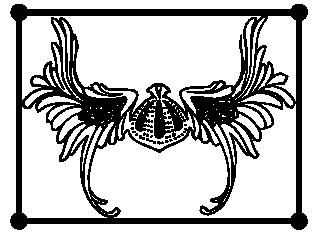
\includegraphics[scale=1.5]{chapter2-casque-viking-pstricks}

\caption[Association d'un modèle à une cage] {Association d'un modèle (casque
viking) à une cage de déformation (en noir). Les disques noirs représentent
les sommets de la cage}

\label{DEFMod}
\end{center}
\end{figure}

Les méthodes présentées ci-dessous permettent de réaliser les étapes
d'association d'un modèle à un outil et de déformation d'un modèle. Afin de
les illuster, nous allons déformer un même modèle (Figure \ref{DEFAva}, tiré
de \cite{LLC08}) en utilisant chaque méthode.

\begin{figure}[ht]
\begin{center}
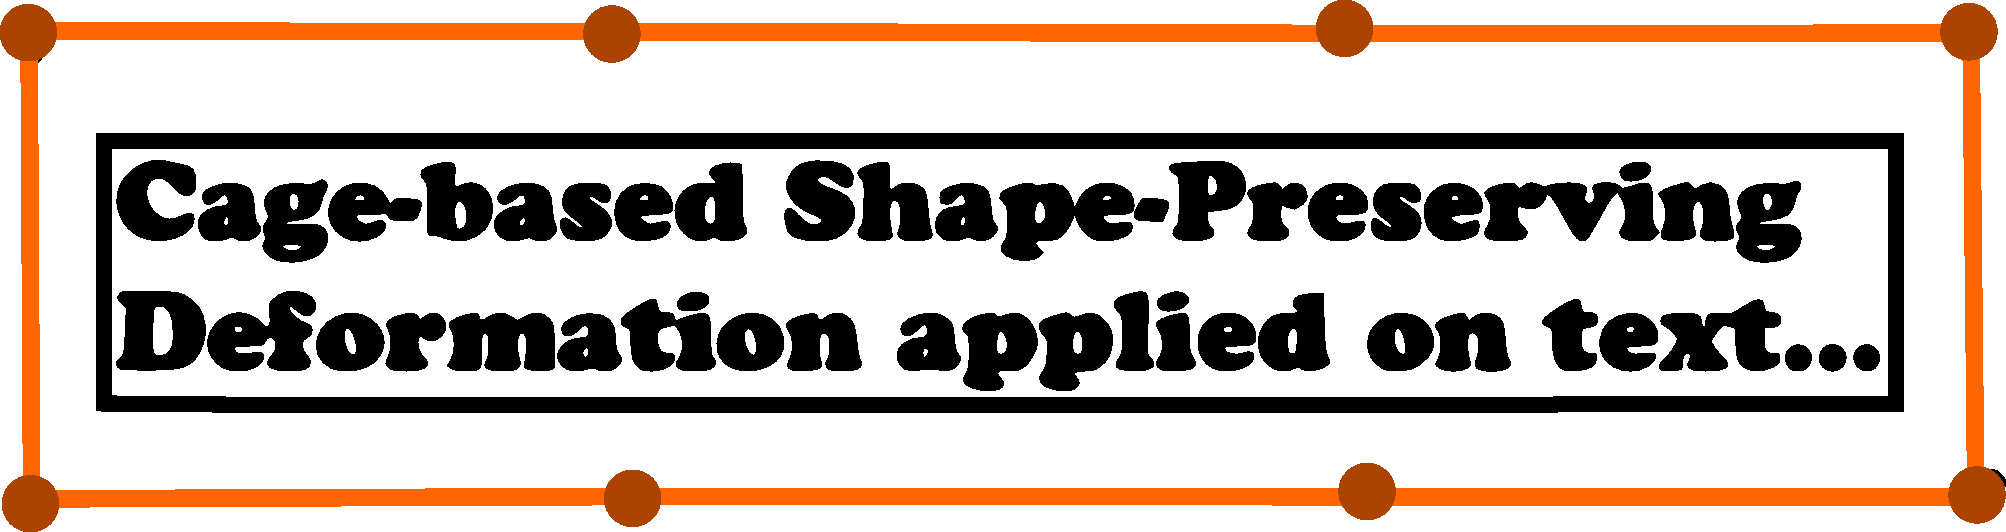
\includegraphics[scale=0.25]{Deformation-Texte-Avant}

\caption[Texte avant déformation] {Texte avant déformation. La cage est
représentée par son bord, en rose.}

\label{DEFAva}
\end{center}
\end{figure}

Les premiers travaux dans ce domaine ont été réalisés simultanément par
\cite{JSW05} \cite{FKR05}, en utilisant la technique des Mean Value
Coordinates (MVC) (développée par \cite{Flo03}). Il s'agit d'utiliser des
coordonnées barycentriques généralisées pour réaliser des déformations. Les
coordonnées barycentriques généralisées correspondent à la généralisation du
calcul de coordonnées barycentriques, en ne considérant plus des coordonnées
calculées par rapport à un simplexe (triangle dans $\mathbb{R}^2$), mais à une
cellule (polygone dans $\mathbb{R}^2$). Néanmoins cette méthode comporte un
important défaut : les coordonnées calculées peuvent être négatives (dans le
cas d'une cage concave par exemple), ce qui peut aboutir à des
résultats contre-intuitifs.

\begin{figure}[ht]
\begin{center}
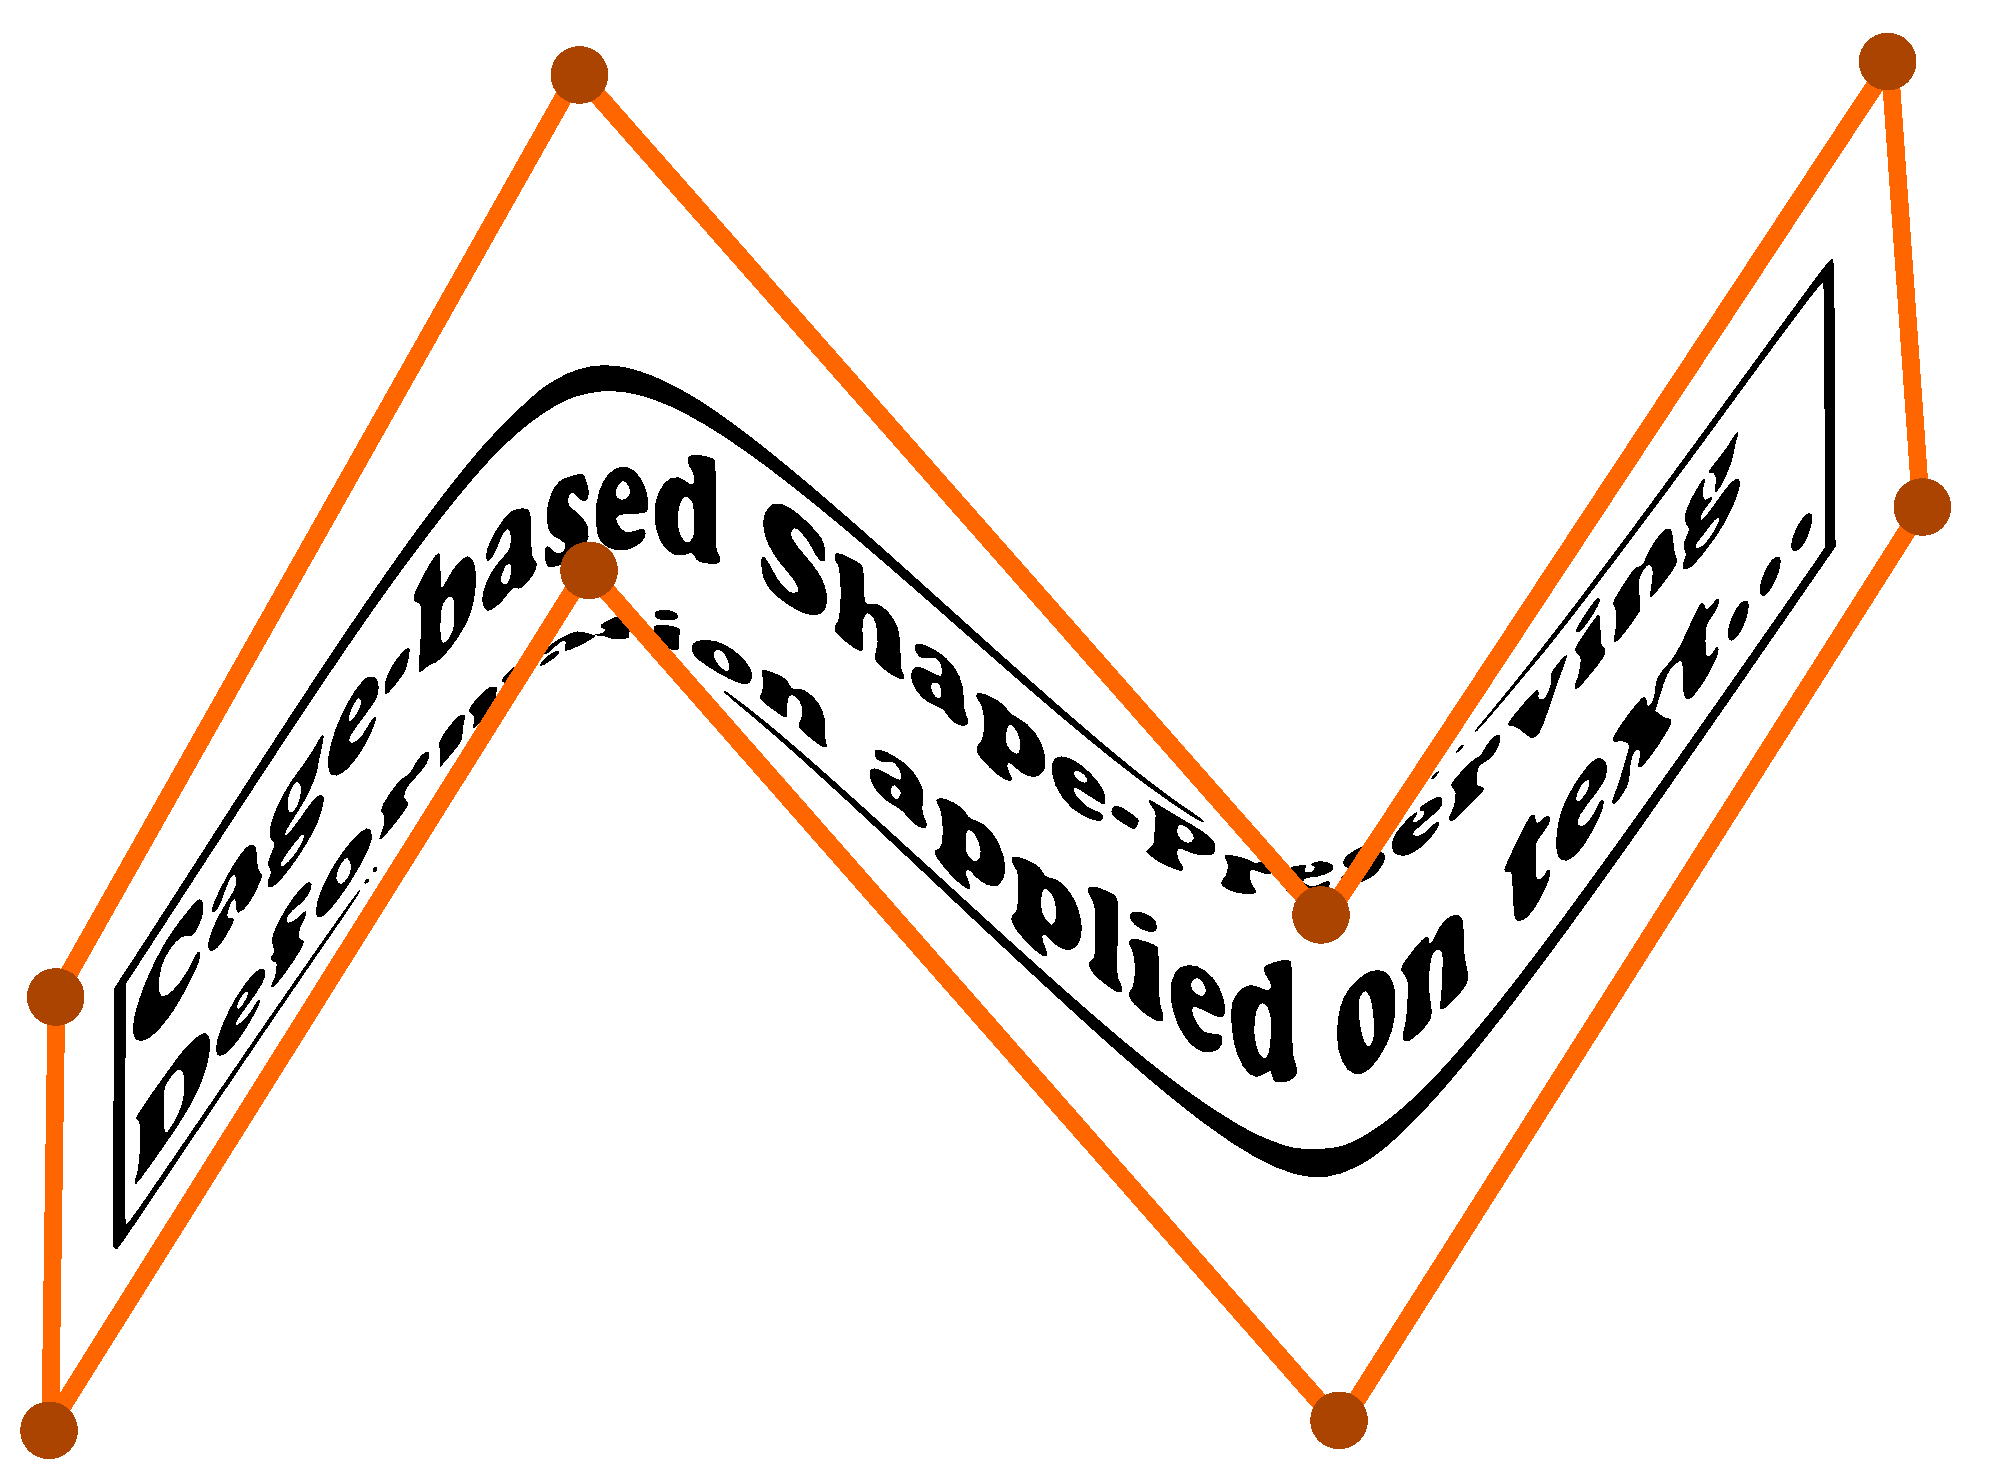
\includegraphics[scale=0.25]{Deformation-Texte-MVC}

\caption[Déformation d'un texte (MVC)] {Déformation d'un texte en utilisant la
méthode des MVC}

\label{DEFMea}
\end{center}
\end{figure}

\cite{JMDGS07} ont déclaré que l'importance de ce problème devait amener à ne
pas utiliser les MVC pour l'animation de personnages. A la place, ils ont
proposé une approche différente, qui ne produisait pas de coordonnées
négatives : les Harmonic Coordinates (Figure \ref{DEFHar}) (Figure. Cette méthode a permis d'obtenir
des déformations plus localisées, au prix d'une complexité en temps de
calcul beaucoup plus importante et d'une discrétisation de l'espace assez
fine.

\begin{figure}[ht]
\begin{center}
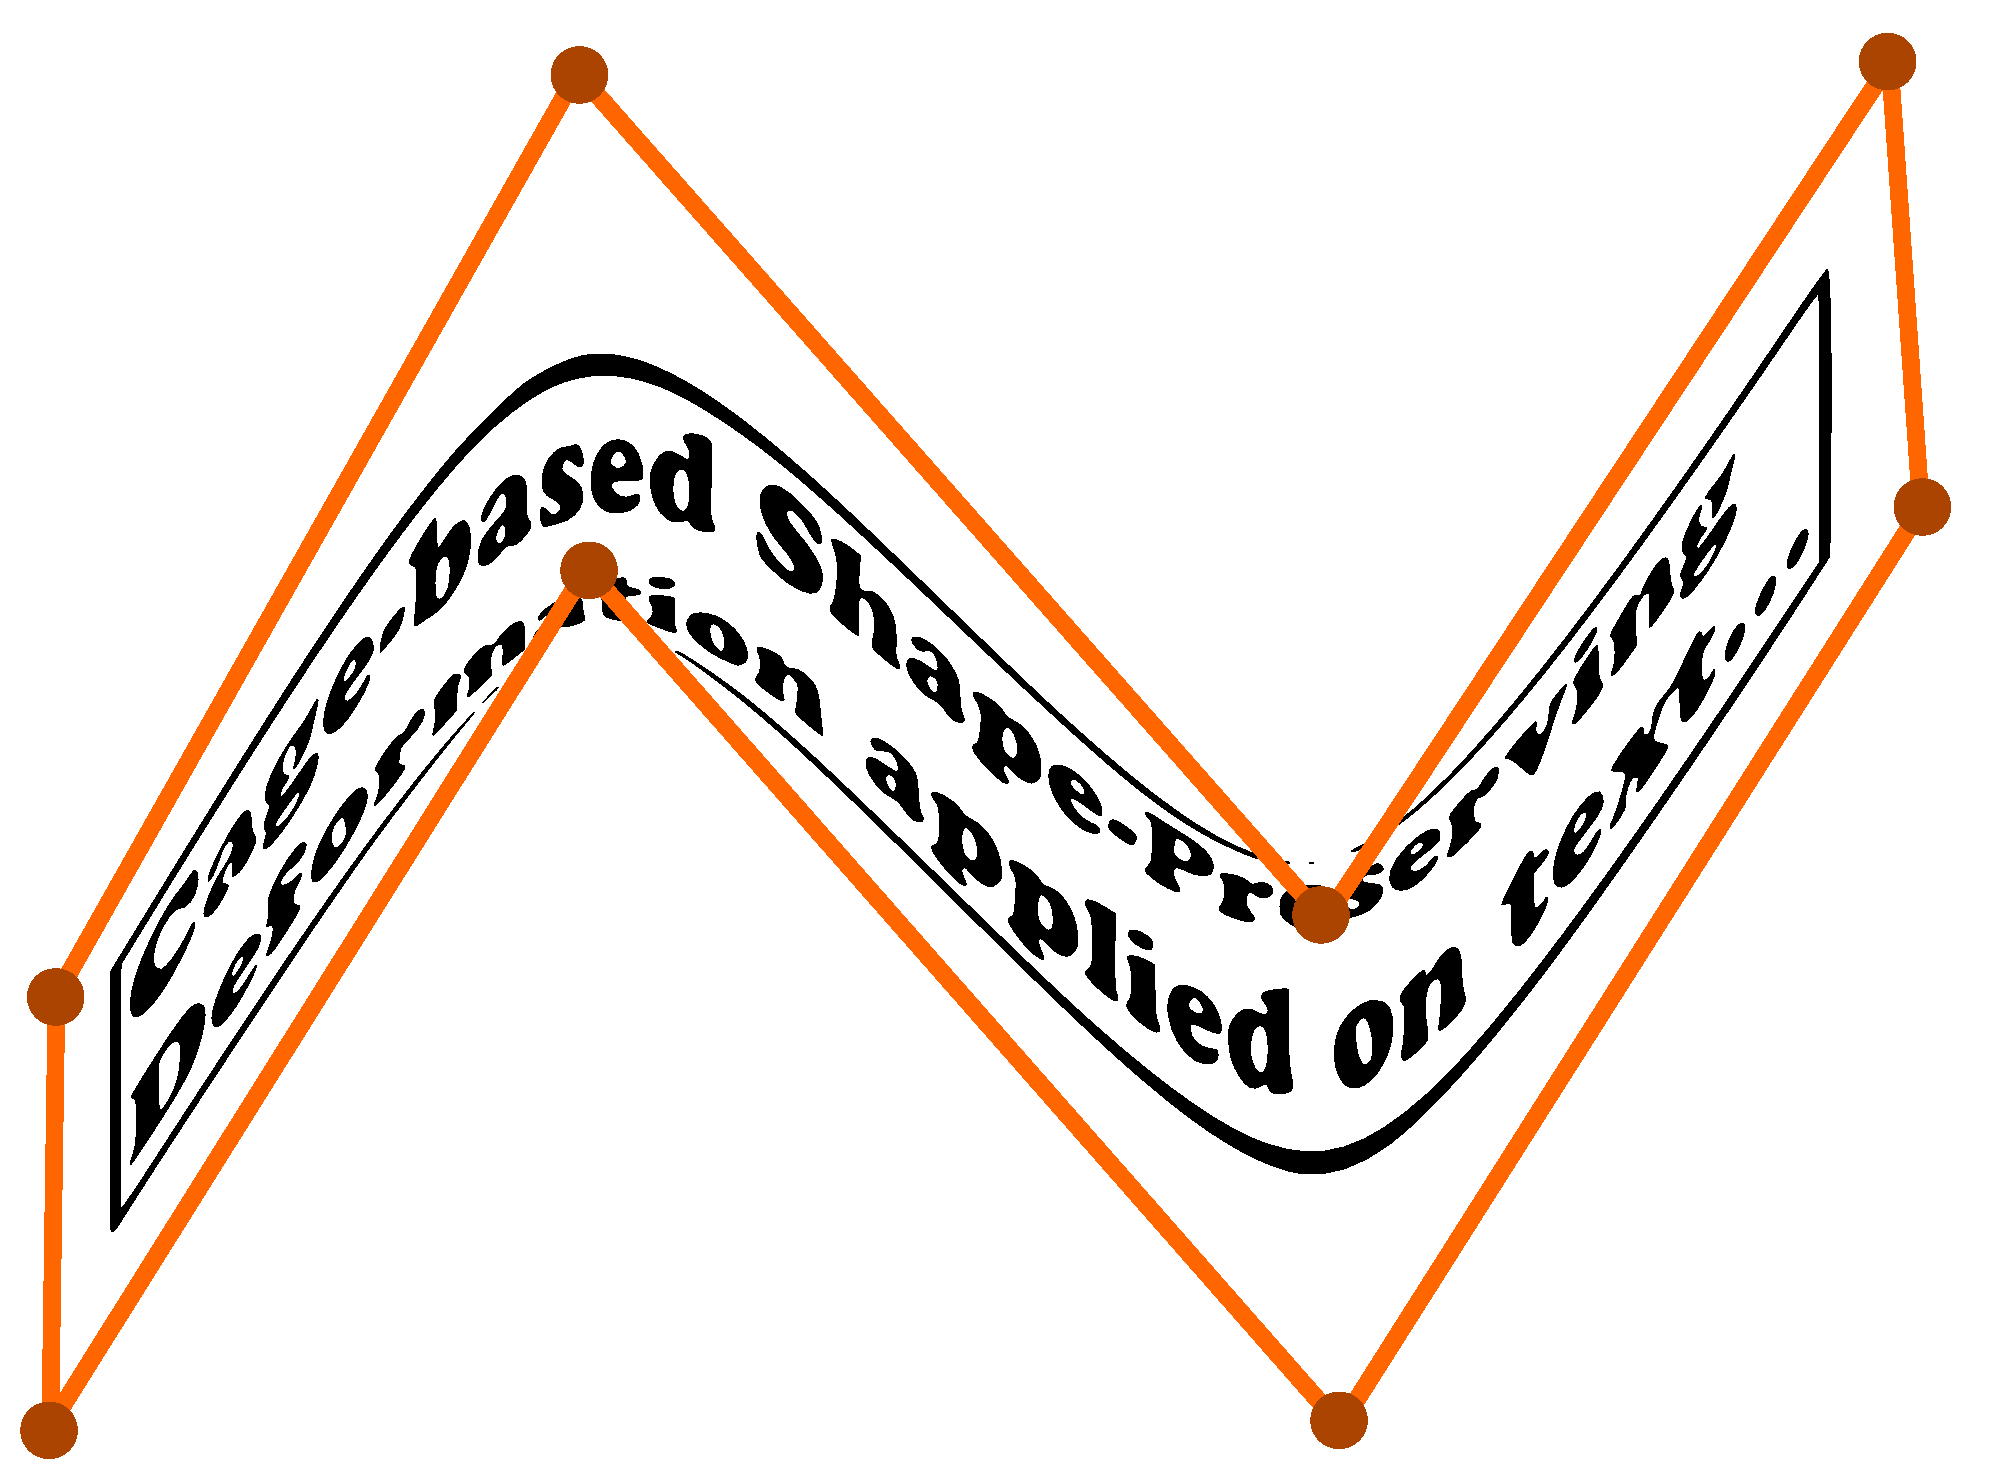
\includegraphics[scale=0.25]{Deformation-Texte-HC}

\caption[Déformation d'un texte (HC)] {Déformation d'un texte en utilisant la
méthode des HC}

\label{DEFHar}
\end{center}
\end{figure}

Dans la même optique, \cite{LKCL07} proposent une amélioration des Mean Value
Coordinates qui les rend positives. L'idée est de se baser sur un test de
visibilité lors du calcul des coordonnées. Ils ont pu obtenir des résultats
similaires à \cite{JMDGS07} pour une complexité en temps de calcul proche de
celle des MVC. \cite{LLC08} ont constaté que les détails de la surface
n'étaient pas préservés, en particulier lors de déformations importantes. Ce
qui les a amené à développer une approche considérant plus de données lors de
l'association du modèle à la cage : les Green Coordinates (GC) (Figure
\ref{DEFGre}). Au lieu d'utiliser uniquement la position des sommets de la
cage, les Green Coordinates utilisent aussi les normales aux faces de la cage.

\begin{figure}[ht]
\begin{center}
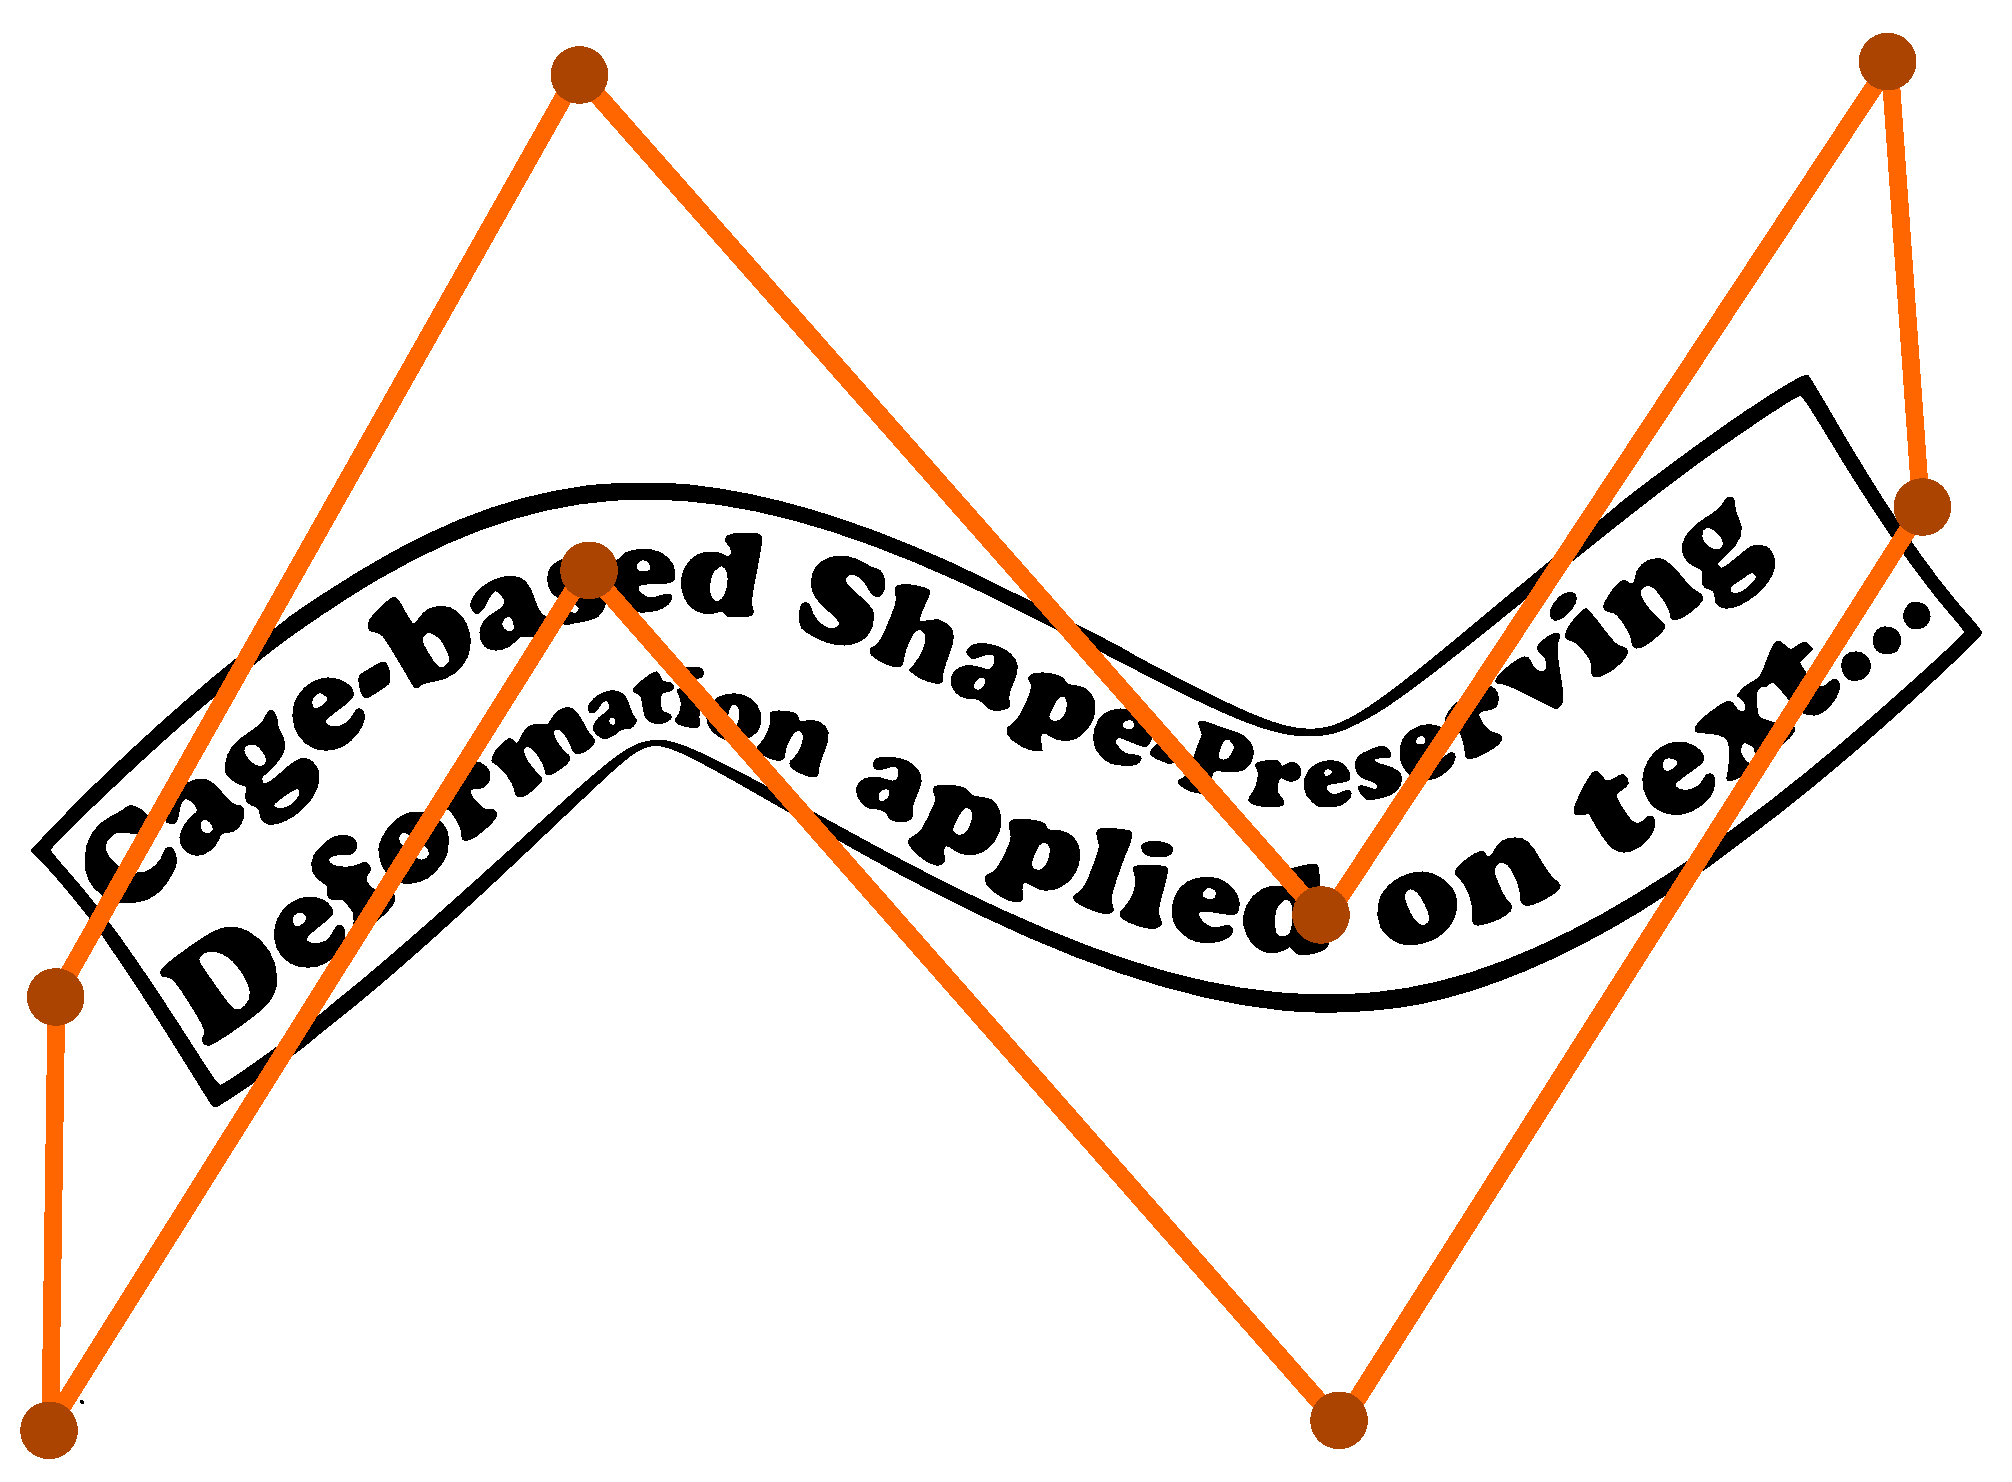
\includegraphics[scale=0.25]{Deformation-Texte-GC}

\caption[Déformation d'un texte (GC)] {Déformation d'un texte en utilisant la
méthode des GC}

\label{DEFGre}
\end{center}
\end{figure}

\section{Mean Value Coordinates}

Dans le cadre de notre travail, nous avons choisi de travailler avec une seule
méthode de calcul des coordonnées. Le choix que nous avons fait s'est porté
sur les MVC. C'est actuellement la méthode de calcul des coordonnées qui a la
plus faible complexité en temps de calcul. De plus, ayant déjà travaillé sur
cette méthode, nous avions déjà fait une première implémentation de la
méthode. La réutiliser nous permet de plus concentrer notre travail sur la
partie mélange de coordonnées. Néanmoins, la méthode apportée par notre
travail ne se limite pas aux coordonnées MVC, mais peut être généralisée à
d'autres méthodes de calcul de coordonnées qui partagent des propriétés en
commun.

\subsection{Coordonnées barycentriques}

\cite{Mob27} a été le premier à exprimer une relation entre un triangle et un
point contenu à l'intérieur de celui-ci : les
coordonnées barycentriques.

Soit $V = \{v_1, v_2, v_3\}$ un triangle quelconque, ses sommets constituent ce
qu'on appelle un repère barycentrique, et soit $p$ un point de l'espace. On dit
que $p$ est un barycentre de $V$ si et seulement si:

\begin{equation}
  p = \frac{w_1 v_1 + w_2 v_2 + w_3 v_3}{w_1+w_2+w_3},
\end{equation}

où $w_i$ correspond à la coordonnée du point $p$ associée au sommet $v_i$,
pour $i \in \{1, 2, 3\}$. On peut réécrire cette formule en normalisant les
$w_i$ :

\begin{equation}
  \lambda_i = \frac{w_i}{w_1+w_2+w_3} ~, i \in \{1, 2, 3\}, 
\end{equation}

et donc $\sum_{i=1}^3 \lambda_i = 1$. On obtient la formulation suivante :

\begin{equation}
  p = \lambda_1 v_1 + \lambda_2 v_2 + \lambda_3 v_3.
\end{equation}

\subsection{Coordonnées barycentriques généralisées}

Soit $V = \{v_1, v_2, ..., v_n\}$ un polygone sans auto-intersection et non-
dégénéré, ses sommets constituent un repère barycentrique. Soit $p$ un
point de l'espace. Le but est d'étudier les poids $\lambda_i$ tels que :

\begin{equation}
  p = \sum_{i=1}^{n} \lambda_i v_i ,
  ~ \forall i \in \mathbb{N} ,~ 1 \leq i \leq n
\end{equation}

où $\lambda_i$ est la coordonnée (normalisée) du point $p$ associée au sommet
$v_i$ et vérifie :

\begin{equation}
  \lambda_i = \frac{w_i}{\sum_{j=1}^n w_j},
\end{equation}

de même que pour les coordonnées barycentriques $\sum_{i=1}^n \lambda_i = 1$.
\\

Le calcul des coordonnées $w_i$ n'est plus aussi évident que pour le cas du
triangle. Contrairement aux coordonnées barycentriques, les coordonnées
barycentriques généralisées ne sont pas uniques. Plusieurs méthodes ont été
mises en place, et nous nous sommes intéressés particulièrement au travail de
\cite{Flo03}.

\subsection{Calcul des coordonnées}

Sa motivation a été de reproduire le comportement de fonctions harmoniques.
Une fonction $u$ définie dans un plan $\Omega \in \mathbb{R}^2$ est dite
harmonique si elle est $C^2$ et qu'elle satisfait l'équation de Laplace :

\begin{equation}
  \frac{\partial^2 u}{\partial x^2} + \frac{\partial^2 u}{\partial y^2} = 0.
\end{equation}

Les fonctions harmoniques n'ayant pas de forme analytique, une manière de
connaître leur valeur en un points précis est de les évaluer sur tout le
domaine. Ces traitements nécessitent beaucoup de calculs, c'est pour cela que
\cite{Flo03} a décidé de les approximer au travers de fonctions linéaires
définies par morceaux sur une triangulation donnée.

La coordonnnée $w_i$ associée au point $p$ est calculée en utilisant la
position du point $p$, du sommet $v_i$ et des deux sommets adjacents à $v_i$ :
$v_{i-1}$ et $v_{i+1}$ (Figure \ref{DEFcal}).

\begin{figure}[ht]
  \begin{center}
    \includegraphics[scale=0.9]{chapter2-pstricks.pdf}

    \caption[Méthode de calcul MVC] {Méthode de calcul de la coordonnée $w_i$
du point $p$ par rapport au sommet $v_i$}

    \label{DEFcal}   \end{center} \end{figure}

La méthode détermine la coordonnée $w_i$ de la manière suivante :

\begin{equation}
  w_i = \frac{tan(\alpha_{i-1}/2) + tan(\alpha_i/2)}{\| v_i - p \|}.
  \label{DEFcoo}
\end{equation}

Ces coordonnées sont ensuite normalisées :

\begin{equation}
  \lambda_i = \frac{w_i}{\sum_{j=1}^n w_j},
\end{equation}

afin d'obtenir la coordonnée MVC du point $p$ par rapport au sommet $v_i$. On
appelle les coordonnées MVC du point $p$ l'ensemble de ces coordonnées
$\{\lambda_0, \lambda_1, ..., \lambda_n\}$.

% Une fois ces calculs effectués, la déformation se réalise par invariance de
% l'association entre le modèle et l'outil. La modification de la position des
% sommets de la cage modifie donc la position des points de l'espace (Figure
% \ref{DEFCom}).

% \begin{figure}
% \begin{center}
% \includegraphics{casque-viking}

% \caption[Deformation à base de cage (MVC)] {Déformation d'un modèle (casque
% viking) par rapport à la modification d'un sommet de la cage associée (en
% noir). A gauche le modèle avant déformation, à droite le modèle après
% déformation.}

% \label{DEFCom}
% \end{center}
% \end{figure}

Ces formules sont correctes dans le cas où un point $p$ est strictement inclus
dans la cage : $p$ n'appartient à aucune arête de la cage. Des problèmes se
posent lorsqu'un point de l'espace se trouve le long d'une arête de la cage.
On peut détecter cette situation en regardant la valeur des angles
$\alpha_{i-1}$ et $\alpha_i$. Par exemple, quand le point $p$ se situe sur
l'arête $E = [v_i,v_{i+1}]$, l'angle $\alpha_i$ vaut $\pi$ (Figure
\ref{DEFinc}). Or :

\begin{displaymath}
  \lim\limits_{x \to \pi^-} tan(\frac{x}{2}) = +\infty
\end{displaymath}

\begin{figure}[ht]
  \begin{center}
    \includegraphics[scale=0.9]{chapter2-pstricks-2.pdf}

    \caption[Cas particulier MVC] {Situation dans laquelle les
formules de calcul de coordonnées ne sont plus correctes.}

    \label{DEFinc}
  \end{center}
\end{figure}

Cela pose un problème par rapport au calcul donné par l'équation \ref{DEFcoo}.
Les coordonnées barycentriques généralisées établissent que les coordonnées
calculées varient de façon linéaire le long des arêtes de la cage et qu'elles
respectent la propriété de Lagrange aux sommets de la cage: Si $p = v_i$ alors
$\lambda_i = 1$ et $\lambda_j = 0 ~\forall~ j \neq i$

En utilisant ces propriétés, on définit un calcul de coordonnées spécifique
pour les points se trouvant le long d'une arête. Pour calculer la coordonnée
$w_j$ du point $p$ par rapport au sommet $v_j$, $p$ se trouvant le long de
l'arête $E = [v_i,v_{i+1}]$, on distingue deux cas :

\begin{itemize}

\item Soit $v_j$ n'est pas incident à $E$ ($v_j \neq v_i$ et $v_j \neq
v_{i+1}$); dans ce cas $\lambda_j = 0$

\item Soit $v_j$ est incident à $E$ ($v_j = v_i$ ou $v_j = v_{i+1}$); dans ce
cas $\lambda_j$ est calculé comme étant le coefficient associé au sommet $v_j$
lors du calcul du barycentre du segment E, en considérant $p$ comme étant le
barycentre.

\end{itemize}